\documentclass[11pt]{article}

\usepackage[latin1]{inputenc}
\usepackage[T1]{fontenc}
\usepackage[spanish]{babel}
\usepackage{apacite}

\decimalpoint

\usepackage{amssymb}
\usepackage{amsbsy}
\usepackage{amsmath}
\usepackage{latexsym}%,pstricks,color,epic,eepic}
\usepackage{multicol}
\usepackage{tikz-cd}
\usepackage[all]{xy}
%\usepackage{titling}
\usetikzlibrary{cd}

\usepackage{lastpage,fancyhdr,graphicx}
\usepackage{epstopdf}
%\pagestyle{myheadings}
\pagestyle{fancy}
\fancyhf{}
%\setlength{\headlengtht}{500pt}
\renewcommand{\headrulewidth}{0.5pt}
\fancyheadoffset[R]{0cm}
\lhead{
\includegraphics[width=2.0in]{LOGO_FINGUACH.png}\hfill {\thepage}}
\lfoot{\tiny Citar como: P. Autor-Uno; et al.; titulo, Fing-UAch num 16 vol 34 enero-junio 2020, o el DOI: o la p�gina etc....}

\setcounter{page}{16}
\hoffset = -50pt
\voffset = -50pt
\textwidth = 500pt
\textheight = 615pt

% Keywords command
\providecommand{\keywords}[1]
{
  \small	
  \textbf{\textit{Keywords---}} #1
}

\def\IR{{\rm I\!R}}  %for real numbers
\def\IN{{\rm I\!N}}  %for integer numbers
\def\IC{{\rm C}\llap{\vrule height7.1pt width1pt
     depth-.4pt\phantom t}} %for complex numbers \def\covD{{\rmI\!D}}
\def\IQ{{\rm Q}\llap{\vrule height7.7pt width1pt
     depth-.4pt\phantom t}} %for complex numbers \def\covD{{\rmI\!D}}

%   Si pones en tus definiciones las siguientes instrucciones:

\font\cmss=cmss10
\font\cmsss=cmss10 at 7pt

\def\IZ{\relax\ifmmode\mathchoice
{\hbox{\cmss Z\kern-.4em Z}}{\hbox{\cmss Z\kern-.4em Z}}
{\lower.9pt\hbox{\cmsss Z\kern-.4em Z}}
{\lower1.2pt\hbox{\cmsss Z\kern-.4em Z}}\else{\cmss Z\kern-.4em Z}\fi}

%   podr'as usar  $ \IZ $  para denotar los enteros.

\def\abs_ing{{\rm }}
\setlength{\parskip}{1em}

\makeatletter
\let\@fnsymbol\@arabic
\makeatother



%---------------*******************************------------------------

% Definition of title page:
\title{
\includegraphics[scale = 0.4]{LOGO_FINGUACH.png}\\
El t�tulo del art�culo}

\author{Primer Autor-Uno
\thanks{Datos de afiliaci�n de cada uno de los autores en el aorden en el que aparecen arriba. Por ejemplo:  Facultad de ciencias de la 
universidad desconocida, avenida universidad \# 6783, Prados de la universidad CP 26345, Timbuktu, Mexico. (e-mail: pa-u@udat.edu.mx)}~\textsuperscript{,}\footnote{corresponding author}
\and
Segundo Autor Dos
\thanks{Rice University, Houston, TX 77005 USA. He is 
now with the Department of Physics, Colorado State University, Fort Collins, 
CO 80523 USA.}
\and
Tercer Autor Tres\footnotemark[1]
}

%\thanksmarkseries{arabic}

%\pagestyle{headings}
\date{1 de enero de 2020\footnote{En este p�rrafo estar� la fecha de primer envio del art�culo a la revista para su revisi�n. Por ejemplo:
 primer envio 10 de agosto de 2019.}.}
 %

\begin{document}

\maketitle

%\hline
\hrulefill
\\
{\centering {\sc Resumen}\\}
{\it  El resumen debe ser menos de 250 palabaras, enfatizando la importancia del trabajo y los resultados obtenidos. es importante mencionar que en esta secci�n el resumen es en espa�ol.}
\vskip 1em

{\centering {\sc  Abstract}\\}
{\it Here goes the abstract in English no more than 250 words, emphasizing the importance of work and the results obtained. this should match with the abstract in spanish.}

%\hline
\hrulefill\\

\keywords{Uno, Dos, Tres, Cuatro, etc}

%\begin{multicols}{2}

\section{Introducci�n}

Aqui se empieza el texto del articulo dividiendo en secciones, subsecciones, el texto matem�tico va en de la forma $f(x) = x^2+3xy$ en donde se 
debe de  $0 \leq x\leq 7$ como ejemplos de texto matem�tico

\begin{eqnarray}
\label{eq:schemeP}
	\mathrm{P_Y} = \underbrace{H(Y_n) - H(Y_n|\mathbf{V}^{Y}_{n})}_{S_Y} + \underbrace{H(Y_n|\mathbf{V}^{Y}_{n})- H(Y_n|\mathbf{V}^{X,Y}_{n})}_{T_{X\rightarrow Y}},
\end{eqnarray}


De preferencia todas las ecuaciones que esten en el ambiente de equation, si no es referenciada incluir el asterisco, solo las ecuaciones que referenciadas van numeradas como la ecuaci�n~\eqref{eq:dos}. La ecuaciones referenciadas se referencian con el comando eqref. 


\begin{equation*}
\begin{tikzcd}[column sep=small, row sep=tiny]
& P \ar[r, Rightarrow] & (P \ar[r, Rightarrow] & Q ) \\
& C \ar[drr, bend right = 95, dash]      & C \ar[r, bend right = 90, dash]  & C \\
&   													   &                  & \parbox{0.5cm}{\flushleft C} \\
&  &\parbox{0.5cm}{\flushright C} &
\end{tikzcd}
\end{equation*}


ahora una mas grande:

\begin{equation}
\begin{tikzcd}[column sep=small, row sep=tiny]
& ((P \parbox{0.5cm}{\centering$\wedge$} & Q)\ar[r, Rightarrow] & B) \ar[r,Rightarrow]   & (P \ar[r, Rightarrow] & (P \ar[r, Rightarrow] & Q )) \\
& C \ar[r, bend right = 90, dash] & C &  F & C \ar[dr, bend right = 95, dash]      & C \ar[r, bend right = 90, dash]  & F \\
& \parbox{0.5cm}{\flushright F} \ar[dr, bend right = 95, dash] &  & 									   &                  & \parbox{0.5cm}{\flushleft F} \\
& & F & &  &\parbox{0.5cm}{\flushright F} &
\end{tikzcd}
\label{eq:dos}
\end{equation}

Este es un ejemplo de una tabla. Es importante mencionar que tambi�n se pueden referenciar las tablas de manera cruzada como es el caso de  la tabla~\ref{table1}.


\begin{table}[!ht]
%\begin{adjustwidth}{-2.25in}{0in} % Comentar o quitar para ajustar que el texto y la tabla se ajuste correctamente.
\begin{tabular}{|lll|l||l|l|ll|}
\hline
\multicolumn{4}{|||}{\bf Heading1} & \multicolumn{2}{|l}{\bf Heading2}\\ \hline
$cell_1 row^1$ & cell2 row 1 & cell3 row 1 & cell4 row 1 & cell5 row 1 & cell6 row 1 \\ \hline
$cell_1 row^2$ & cell2 row 2 & cell3 row 2 & cell4 row 2 & cell5 row 2 & cell6 row 2 \\ \hline
$cell_1 row^3$ & cell2 row 3 & cell3 row 3 & cell4 row 3 & cell5 row 3 & cell6 row 3 \\ \hline
\end{tabular}
\caption{Descripci�n de la tabla.}
\label{table1}
%\end{adjustwidth}
\end{table}

\section{M�todos y materiales}


En esta secci�n poner los materiales y m�todos empleados. a continuaci�n se pone una gr�fica de muestra ver Figura~\ref{fig1}.

\begin{figure}[hbt]
\centering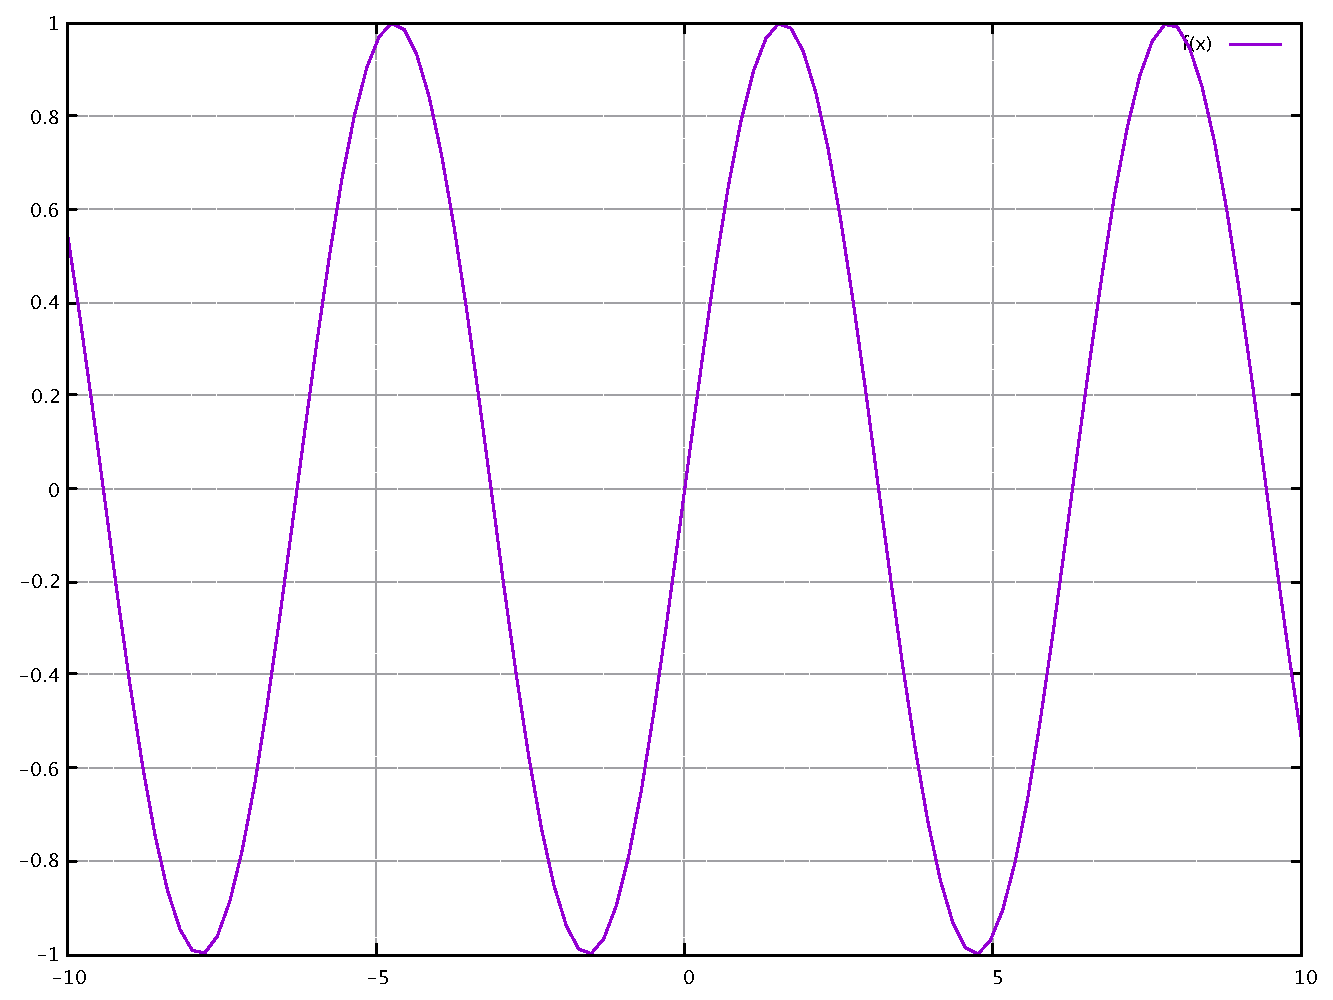
\includegraphics[scale=0.5]{imagen1}
\caption{{\bf funci�n $\sen(x) $ en negritas titulo de la figura.} Descripci�n de la figura.}
\label{fig1}
\end{figure}

Determina el dominio de analiticidad de la funci�n y calcula $\displaystyle \int_\gamma f(z) dz $, donde $\gamma$ es el c�rculo unitario centrado en cero. Cuando $f(z)$ es:
\begin{enumerate}
 \item $f(z) = \displaystyle\frac{z^2}{z-3}$
 \item $f(z) = \displaystyle z e^{-z}$
 \item $f(z) = \tan(z)$
\end{enumerate}


\section{Resultados}



La corriente $I(t)$ en un circuito LC en serie queda descrita por:
\begin{equation*}
 I''(t)+5I'(t)+6I(t)=\begin{cases}
                      0 & 0 \leq t \leq 1\ ; \\
                      t & 1 < t < 5 \ ; \\
                      1 & 5 < t\ .
                     \end{cases}
                     \quad I(0) =0; I'(0)=2\ .
\end{equation*}
Determinar la corriente en funci�n del tiempo y hacer un bosquejo de $I(t)$ para $0<t<6$.

Aqu� un ejemplo de alineaci�on de ecuaciones
\begin{align}
 f(x) &= x^4 + 7x^3 + 2x^2 \nonumber \\
      &\qquad {} + 10x + 12
\end{align}


\section{Conclusi�n}
La bibliografia, lo m�s recomendable es manejar BibTeX~\cite{chialvo}, en ese caso solo es necesario indicar el nombre del archivo bib en el cual est� la bibliografia~\cite{plenz}, es importante mencionar que tipicamente en el archivo bib es necesario usar UTF8 enconding (se pueden presentar problemas con los acentos y otros s�mbolos de escritira ajenos al ingl�s~\cite{Coolenbook}.)

\section*{Ap�ndices}

Aqu� van los ap�ndices en caso de ser necesarios

\section*{Agradecimientos}

Evitar expresiones como  ``Uno de nosotros (S.A.D) desea dar las gracias $\ldots$ .'' En su lugar escribir  ``P. A. Autor agradece  $\ldots$ .'' 
\textbf{En negritas los agradecimientos a patrocinadores y datos de becas.}


\bibliographystyle{apacite}
\bibliography{biblio}
%\end{multicols} 
 
%
%\begin{thebibliography}{99}
%\bibitem{1}  Calculo; Robert T. Smith, Roland B. Minton; McGraw Hill; 2000.
%\bibitem{2}  Calculo diferencial e integral; Frank Ayres Jr:, Elliot Mendelson; McGraw Hill ;3ra Edicion.
%\bibitem{3}  Calculo una variable; Thomas; Editorial Pearson; und�cima edici�n.
%\bibitem{4}  El calculo con geometr�a anal�tica; Louis Leithold; editorial Harla; 6ta edici�n; a�o 1992.
%\end{thebibliography}

\end{document}
